\documentclass[rnd]{mas_proposal}

\usepackage[utf8]{inputenc}
\usepackage{amsmath}
\usepackage{amsfonts}
\usepackage{amssymb}
\usepackage{graphicx}
\usepackage{float}
\usepackage{array}

\title{Comparative Study: Uncertainty Estimation for Quantized Deep Learning based Classification Models}
%Comparative Study: Model Uncertainty for Quantized Deep Learning based Classification Models
%A comparative study of uncertainty estimation for image processing models in deep learning accelerators

%Footer title in line 198 of mas_proposal.cls file
\author{Mohan Raj Nadarajan}
\supervisors{Prof. Dr. Sebastian Houben\\M.Sc. Deebul Sivarajan Nair}
\date{December 2022}


\begin{document}
\maketitle
\pagestyle{plain}
\section{Introduction}
In applied machine learning, the effectiveness of deep learning based classification models over other conventional machine learning models is indisputable. Though the deep learning models  exhibits higher accuracy, the wrong predictions are with higher value of confidence, which will not only fail the task, but also put human lives at jeopardy in the case of safety critical and real world applications\cite{gawlikowski2021survey}. As a result, it is very important for the deep learning practitioners to be aware of the uncertainty estimates. The basic neural network architecture provides only the predictions and does not capture it's uncertainty\cite{dropout}. 
\begin{figure}[h!]
    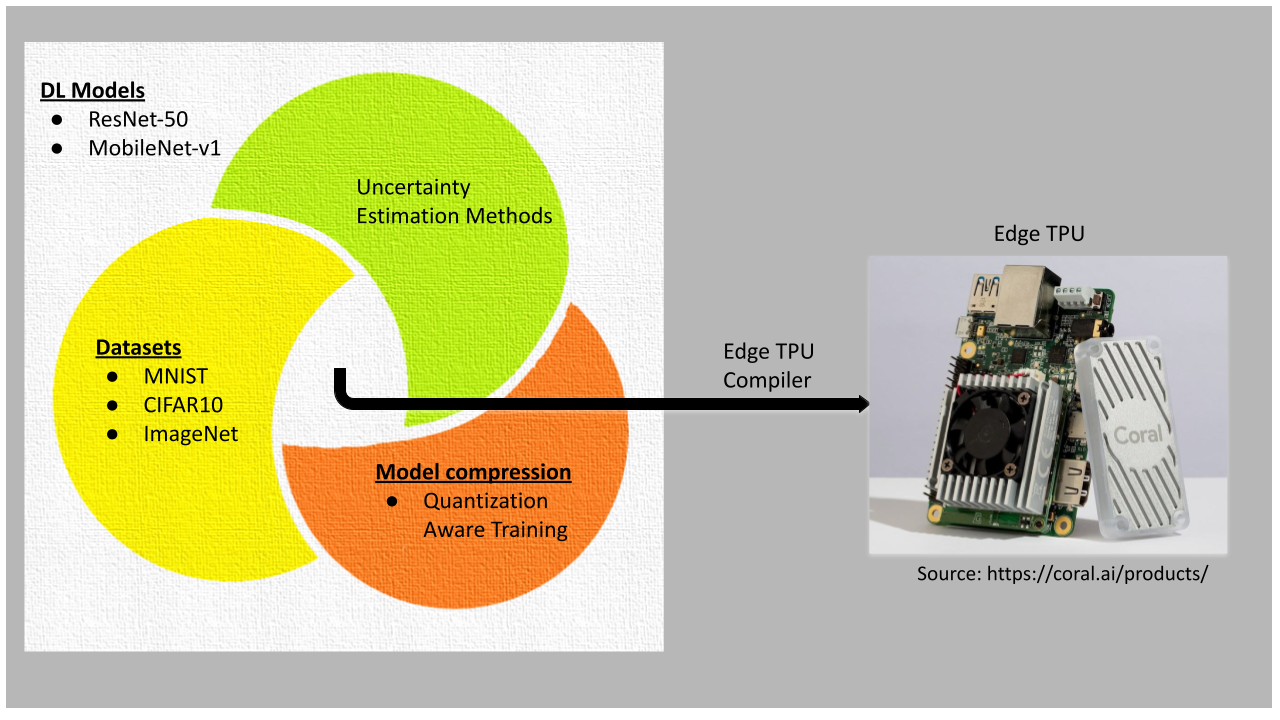
\includegraphics[width=\textwidth]{images/VennDiagram_V1.png}
    \caption{Project components}
    \label{fig:myfigure}
\end{figure}
\\
The predictive uncertainty in a deep learning model is of two types aleatoric uncertainty and epistemic uncertainty or a combination of both\cite{ue_qunatification}. Aleatoric uncertainty also known as data uncertainty is due to the noise in the training data. Epistemic uncertainty also known as model uncertainty is due to uncertainty in the parameters of the model. The epistemic type of uncertainty can be reduced with increase in data provided to the model. The state of the art uncertainty estimation methods for deep learning models has provided techniques like Monte Carlo dropout, stochastic batch normalization, test-time data augmentation, deep ensembles, softmax calibration, selective classification, deterministic and evidential approaches.
\\\\
Edge AI combines artificial intelligence and edge computing. The advancements in edge devices for AI applications to make real time insights along with improved privacy, reduced latency and high availability is revolutionizing the world's largest industries and expanding business outcomes across all sectors. Edge AI runs on a wide range of hardware from microcontroller to tensor processing devices for real world applications like smart watches, autonomous cars, mobile phones.
\\\\
Training or inferencing the neural network algorithms on general purpose hardware like CPU (von Neumann architecture) or GPU is inefficient due to higher number of multiply-accumulate operations\cite{hubara2017quantized}. One way to accelerate neural network workload is using the specialized matrix processor called Tensor Processing Unit. They are of domain specific hardware architecture for deep learning and is a combination of matrix multiplication unit (MXU), vector processing unit and high-bandwidth memory. The MXU contains series of multiply-accumulators, connected directly to each other forming a systolic array architecture. 
\begin{figure}[h!]
    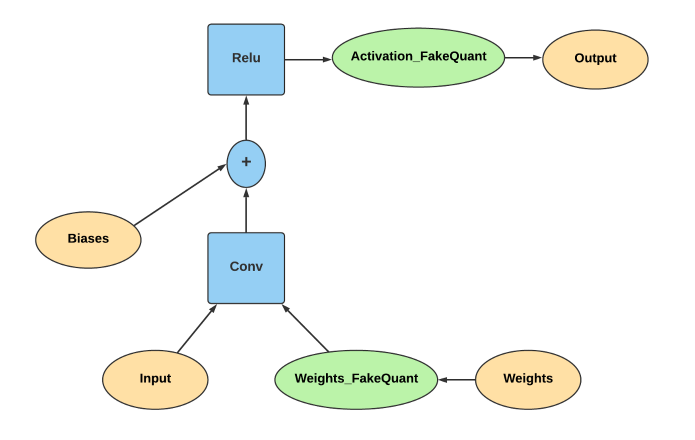
\includegraphics[width=\textwidth]{images/QAT.png}
    \caption{Quantization-aware Training. Duplicated from \cite{qunatifi}}
    \label{fig:myfigure}
\end{figure}
\\
Most of the edge TPUs supports only network compressed deep learning model, in order to accelerate the performance of neural network workloads. The popular compression technologies are quantization, pruning and knowledge distillation. Quantization is the process of lowering compute demand by converting 32-bit representation of parameter data into lower representations like 8-bit, 16-bit or others to make the model more compatible with edge device hardware architecture. This helps to achieve a maximum of 4X improvements in memory, significantly reducing the number of transistors required in the chip. The three types of quantization methods are Quantization-aware Training(QAT), Post-Training Static Quantization(PTQ) and Post-Training Dynamic Quantization. QAT uses "fake quantized" nodes in forward backward passes to simulate the impact of lower bit representation during training and is more accurate than post training quantization methods.
\\\\
The deep learning based image classification task using edge devices is widely used in applications like robotics, health care and industrial machines like quality inspection, metrology and packaging. However, the state of the art uncertainty estimation methods for the deep learning models does not guarantee to provide same results for quantized and non-quantized models. Hence, this project is to evaluate the uncertainty estimates between quantized and non-quantized deep learning models and between multiple quantized deep learning models with different uncertainty estimation techniques.
\begin{figure}[h!]
    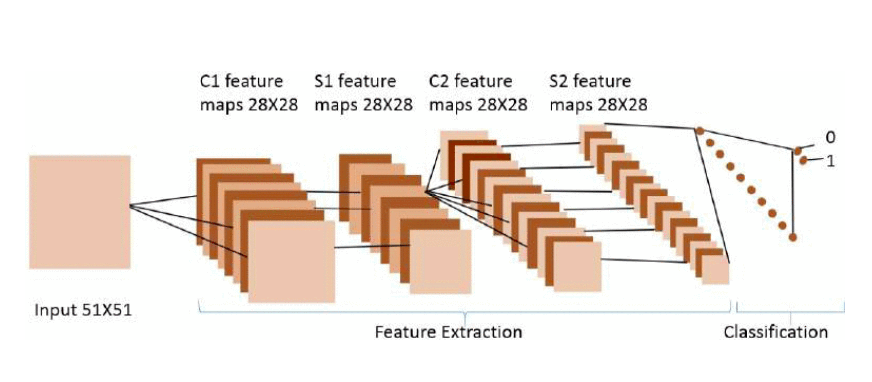
\includegraphics[width=\textwidth]{images/DNN.png}
    \caption{Deep neural network. Duplicated from \cite{DNN_Picture}}
    \label{fig:myfigure}
\end{figure}
\\\\
\textbf{Why is it important?} \\
Institutions from every industry is trying to boost automation for enhancing workflow, productivity, and safety with a range of tasks in unstructured world using edge AI. The deep learning model based inference engines deployed on edge devices makes decision for real-world questions. So it is important to study the uncertainty estimates for quantized model. This helps in the risk assessment for the decisions to be made for the model's prediction. The incorrect predictions of the model in safety-critical applications can endanger human lives. For instance, IBM's supercomputer Watson recommended 'incorrect and unsafe' cancer treatments\cite{ibm}. 
\\\\
One of the application uses a deep learning model to classify objects in the KUKA youBot\cite{bischoff2011kuka}, an omnidirectional mobile manipulator for education and research. The neural network workload is deployed on the robot controller hardware itself and due to it's heavier computation power demand, active perception is not possible. This robot is used in RoboCup@Work league and one of the tasks is to pick desired object from multiple station environment. In a scenario, the robot accidentally picked up the wrong object, due to over confident prediction of the deep learning model. However if the uncertainty score is calculated for and along with the model's prediction, a recovery action could have been performed. And deploying this neural network workload in edge device can help to perform active perception with lower latency.
\\\\
As a result, it is important to evaluate for differences in uncertainty estimates between quantized and non-quantized deep learning models. This study helps to ensure the qualitative analysis of deploying the deep learning models on edge devices and to accelerate the growth edge AI applications. 

\subsection{Problem Statement}
The rise in the popularity of edge computing throws new demands to computing platforms with regards to power, performance and energy efficiency. The success or failure of using edge devices for a specific task will ultimately depend on the right tradeoff among these metrics. In safety critical and real world applications such as risk assessment\cite{mackay1995bayesian}, autonomous driving\cite{mcallister2017concrete} and medicine\cite{liang2018bayesian}, the guarantees for decision making while using deep learning models is vital and is required to evaluate the model uncertainty for compressed networks. However, the recent research works evaluates the inference accelerators based on energy consumption for common inference workloads and inference time, which is not sufficient for safety intensive applications. Since quantization reduces model size while also enhancing training latency and inference, it is widely used in comparison with other model compression techniques\cite{rodriguez2018lower}. This R\&D work is to provide an empirical study of the uncertainty estimates for the quantized deep learning models from the perspective of edge computing.

\subsection{Research Questions}
What are the difference in uncertainty estimation metrics for quantized deep learning based classification models with different uncertainty estimation methods?
\begin{itemize}
    \item How does the uncertainty estimates of quantized deep learning model differ from non-quantized deep learning model?
    \item How does evidential loss function impact the QAT?
\end{itemize}


\section{Related Work}
\subsection{Survey of Related Work}
The most common benchmarking metrics of deep learning hardware accelerators are energy efficiency, performance and power. The success or failure of these Domain Specific Architectures (DSA) are determined by these metrics in the state of art evaluations. The measurement terms for energy efficiency, performance and power are in terms of Operations per Watt, time per inference, and Watt respectively. Since the aim of of DSA is to accelerate inference related operations with reasonable power budget, this brings a research question on how reliable the deep learning model predictions are.
\\\\
MLPerf, coalition of artificial intelligence accelerators from industry, academia and research labs, aiming to provide state of the art performance evaluation for training and inference tasks. The internal structure of the MLPerf inference submission system has four components and are system under test(SUT), dataset, load generator(LoadGen), and an accuracy script. The LoadGen is a configuration file which handles the traffic generation, loading data for inference  and measuring performance. The query format created by LoadGen for different scenarios are single stream, multistream, server and offline. In single stream format, the next query is sent only after the completion of previous query. In multi stream format, the set of inferences per query is sent periodically with a  predefined time interval. In server format, the query is random and the SUT responds back within a defined latency limit. In offline format, the whole test data is sent as a batch and latency is not constrained. An empirical study to evaluate the system is performed by MLPerf with ResNet-50 v1.5 and MobileNet-v1 224 models on ImageNet dataset for classification task. The important contribution of this work is to identify the metrics and inference scenarios where AI accelerators are most useful.
\\\\
Achterhold et al. created a complex pruning and quantization strategy for pointwise NNs, but with the help of Bayesian inference\cite{achterhold2018variational}. The author trained a bayesian neural network which is pruning \& quantisation friendly and with improper priors. They later converted it to pointwise NNs to achieve reduced memory, but the final non qunatized bayesian NNs were not able to estimate uncertainty because of improper priors\cite{ferianc2021effects}. This R\&D work is to learn a quantized NN directly and predicting model uncertainty considering a range of uncertainty estimation methods without changes in model architecture.

\section{Project Plan}
\subsection{Work Packages}
The R\&D project contains the following work packages
\begin{enumerate}
    \item[WP1] \textbf{Literature search}
        \begin{itemize}
        \item Literature search on neural network compression methods for deep learning model
        \item Literature search on quantization types for deep learning model
        \item Literature search on estimating uncertainty for deep learning models in classification tasks
        \item Literature search on uncertainty estimation evaluation methods
        \end{itemize}
        
    \item[WP2] \textbf{Experimental setup and analysis}
        \begin{itemize}
        \item Implement ResNet DNN model with quantization technique and widely used uncertainty estimation methods for classification task
        \item Train ResNet model on different datasets like MNIST, CIFAR10, ImageNet for classification task
        \item Implement MobileNet DNN model with quantization technique and widely used uncertainty estimation methods for classification task
        \item Train MobileNet model on different datasets like MNIST, CIFAR10, ImageNet for classification task
        \end{itemize}
        
    \item[WP3] \textbf{Model uncertainty evaluation}
        \begin{itemize}
        \item Performing experiments to estimate ResNet model uncertainty for classification tasks on different datasets like MNIST, CIFAR10, ImageNet
        \item Performing experiments to estimate MobileNet model uncertainty for classification tasks on different datasets like MNIST, CIFAR10, ImageNet
        \item Comparative evaluation of the model uncertainty estimates for classification task for difference in dataset and model
        \end{itemize}
        
    \item[WP4] \textbf{Deployment on Edge device}
        \begin{itemize}
        \item Compilation of the quantized ResNet model with Coral Edge TPU compiler to support deploying it on neural network hardware accelerator, Google Coral - USB Accelerator
        \item Perform an inference query on the edge device and gather the uncertainty estimates to compare with the uncertainty estimation of quantized models deployed on GPU.
        \end{itemize}
        
    \item[WP5] \textbf{Project report}
        \begin{itemize}
        \item Documentation of neural network compression techniques for deep learning models
        \item Documentation of state of the art uncertainty estimation methods for classification task
        \item Documentation of quantized DNN inference engine deployment in the edge device
        \item Documentation of uncertainty estimates for ResNet model on all datasets used in the experiment
        \item Documentation of uncertainty estimates for MobileNet model on all datasets used in the experiment
        \item Documentation of comparative evaluation of the model uncertainty estimates for different uncertainty estimation methods and deep learning models
        \item Documentation of conclusions and recommendations for future work
        \item Draft R\&D report explaining research findings
        \item Final R\&D report explaining research findings
        \end{itemize}
\end{enumerate}

\subsection{Milestones}
    \begin{table}[H]
       \begin{tabular}{|m{0.35cm}|m{4cm}|m{9cm}|}
       \hline
       \textbf{M} & \textbf{Milestone} & \textbf{Checkpoints} \\
       \hline
       1 & Literature search & Read top research papers on uncertainty estimation and quantization techniques for DNN models\\
       \hline
       2 & Experimental setup and analysis & Implement ResNet and MobileNet models with quantization techniques and widely used uncertainty estimation methods for classification task\\
       \hline
       3 & Model uncertainty evaluation  &  Performing experiments to estimate model uncertainty for classification tasks on different datasets\\
       \hline
       4 & Deployment on Edge device & Compilation of quantized deep learning model and deploy it on the edge device to perform inferencing\\
       \hline
       5 & Project report & Document all research findings and submission of final R\&D report\\
       \hline
       \end{tabular}
        \caption{Project milestones}
        \label{tab:my_label}
    \end{table}


\subsection{Project Schedule}
\begin{figure}[h!]
    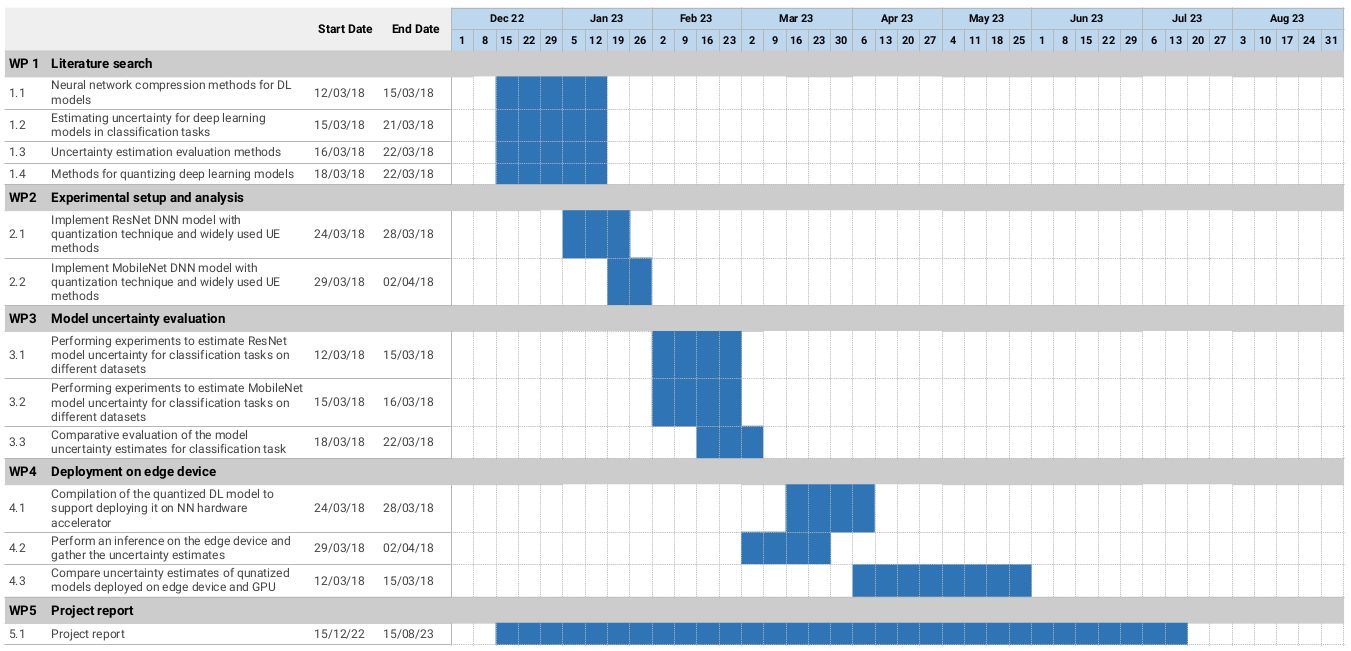
\includegraphics[width=\textwidth]{images/R&D Gantt Chart_V2.png}
    \caption{Project schedule}
    \label{fig:myfigure}
\end{figure}

\subsection{Deliverables}

\subsubsection*{Minimum Viable}
\begin{itemize}
    \item Literature search on neural network compression methods for deep learning model
    \item Literature search on uncertainty estimation evaluation methods
    \item Implementing ResNet and MobileNet models with quantization techniques and widely used uncertainty estimation methods
    \item Train ResNet and MobileNet models on different datasets like MNIST, CIFAR10, ImageNet for classification task
\end{itemize}

\subsubsection*{Expected}
\begin{itemize}
    \item Performing experiments to estimate ResNet model uncertainty for classification tasks on different datasets like MNIST, CIFAR10, ImageNet
    \item Performing experiments to estimate MobileNet model uncertainty for classification tasks on different datasets like MNIST, CIFAR10, ImageNet
    \item Comparative evaluation of the model uncertainty estimates for classification task for difference in dataset and model
    \end{itemize}

\subsubsection*{Desired}
\begin{itemize}
    \item Compilation of the quantized ResNet model with Coral Edge TPU compiler to support deploying it on neural network hardware accelerator, Google Coral - USB Accelerator
    \item Perform an inference query on the edge device and gather the uncertainty estimates to compare with the uncertainty estimation of quantized models deployed on GPU.
\end{itemize}

\nocite{*}
\bibliographystyle{plainnat} 
\bibliography{bibliography.bib}
\end{document}
